%%%%%%%%%%%%%%%%%%%%%%%%%%%%%%%%%%%%%%%%%%%%%%%%%%%%%%%%%%%%%%%%%%%%%
%
%  This is a sample LaTeX input file for your contribution to 
%  the M&C2023 topical meeting.
%
%  Please use it as a template for your full paper 
%    Accompanying/related file(s) include: 
%       1. Document class/format file: mc2023.cls
%       2. Sample PDF/Postscript Figure: figure.pdf,figure.ps
%       3. A PDF file showing the desired appearance: mc2023_template.pdf
%       4. cites.sty and citesort.sty that might be needed by some users 
%    Direct questions about these files to: buijsa@mcmaster.ca
%    Originals provided by brantley1@llnl.gov
%
%    Notes: 
%      (1) You can use the "dvips" utility to convert .dvi 
%          files to PostScript.  Then, use either Acrobat 
%          Distiller or "ps2pdf" to convert to PDF format. 
%      (2) Different versions of LaTeX have been observed to 
%          shift the page down, causing improper margins.
%          If this occurs, adjust the "topmargin" value in the
%          mc2023.cls file to achieve the proper margins. 
%
%%%%%%%%%%%%%%%%%%%%%%%%%%%%%%%%%%%%%%%%%%%%%%%%%%%%%%%%%%%%%%%%%%%%%


%%%%%%%%%%%%%%%%%%%%%%%%%%%%%%%%%%%%%%%%%%%%%%%%%%%%%%%%%%%%%%%%%%%%%
\documentclass[letterpaper]{mc2023}
%
%  various packages that you may wish to activate for usage 
\usepackage{tabls}
\usepackage{cites}
\usepackage{epsf}
\usepackage{appendix}
\usepackage{ragged2e}
\usepackage[top=1in, bottom=1in, left=1in, right=1in]{geometry}
\usepackage{enumitem}
\setlist[itemize]{leftmargin=*}
\usepackage{caption}
\captionsetup{width=1.0\textwidth,font={bf,normalsize},skip=0.3cm,within=none,justification=centering}

%\usepackage[justification=centering]{caption}

%
% Define title...
%
\title{Title of the Paper/Extended Abstract: Centered, Title Case, 14 Point Times \\
  New Roman, on Second Line from the Top Margin,\\ Not
  More Than Three Lines Long}
%
% ...and authors
%
\author{%
  % FIRST AUTHORS 
  %
  \textbf{A.~Author$^1$, B.~Otherauthor$^2$, and C.~Lastauthor$^3$}\footnote{Footnote, if necessary, in Times New Roman font and font size 10}\vspace{3pt} \\
  $^1$Name of Institution 1  \\
  Corresponding Address \vspace{6pt}\\ 
  $^2$Name of Institution 2  \\ 
    Corresponding Address\vspace{6pt} \\ 
  $^3$Name of Institution 3  \\
     Corresponding Address\vspace{6pt} \\
  \url{AuthorA@email}, \url{AuthorB@email}, \url{AuthorC@email}
}
%
% Insert authors' names and short version of title in lines below
%
\newcommand{\authorHead}{Authors' names, use et al.~if more than three}
\newcommand{\shortTitle}{Short One Line Paper Title}
%
%%%%%%%%%%%%%%%%%%%%%%%%%%%%%%%%%%%%%%%%%%%%%%%%%%%%%%%%%%%%%%%%%%%%%
%
%   BEGIN DOCUMENT
%
%%%%%%%%%%%%%%%%%%%%%%%%%%%%%%%%%%%%%%%%%%%%%%%%%%%%%%%%%%%%%%%%%%%%%
\begin{document}
\maketitle
\justify 
\parskip 6pt plus 1 pt minus 1 pt

\begin{abstract}
  Use 8.5"$\times$11" paper size (US letter), with 1'' margins on all sides.  A required 200-250 
  word abstract starts on this line.  Leave two blank lines before ``ABSTRACT''
  and one after.  Use 11 point Times New Roman here and single (11 point) 
  spacing. The abstract is a very brief summary highlighting main 
  accomplishments, what is new, and how it relates to the state-of-the-art.
Both the {\it extended abstract} (2-4 pages, to be submitted for review) and the {\it full paper} (10 pages max, to be submitted for the proceedings) must include this abstract.  
\end{abstract}
\vspace{6pt}
\keywords{list of three to five key words}

\section{INTRODUCTION} 
The full paper as well as the extended abstract start here with two blank lines before first section title.  Use 
8.5"$\times$11" paper size (US letter), with 1'' margins on all sides.  Use one blank line 
before and after each subsequent section's title.  Most of the formatting is globally
set by the specifications given in the \texttt{mc2023.cls} file.  
First-level section titles must be all uppercase and centered, and must 
be numbered in Arabic numerals as shown above.  Unlike the Word template, the body
text and section titles for this \LaTeX\ template use 
11-point font.  We have found that the 11-point font in \LaTeX\ more closely 
matched the 12-point font in Word.  Introduce the topic of the work 
in this section.

The first line of a paragraph is not indented; rather add 6 pt spacing between 
paragraphs.  This is done automatically in the \LaTeX\ template.

There are four types of reference styles: journal paper~\cite{journal}, 
proceedings paper~\cite{proc_paper}, book~\cite{book}, and website~\cite{website}.
References to websites are discouraged. It 
is the author's responsibility to check links in the PDF file of the paper. 
All references should be cited in the text in numerical order, in order of 
appearance as [5-7].

Submission of papers is done in two stages: i) an {\it extended abstract} of length between two and four pages is submitted by the deadline of November 1, 2022 for review; ii) upon acceptance, a {\it full paper} of maximum length of 10 pages is submitted by May 9th, 2023 for inclusion in the proceedings.    
Papers longer than 10 pages
will be billed at \$100/page in excess of 10 pages.  It is strongly recommended
that the length of any final paper should not exceed 12 pages.

\section{SECOND OR SUBSEQUENT MAJOR HEADING} 
\label{sec:first}

This is Section~\ref{sec:first}. It is followed by a subsection, that is, 
\ref{sec:second}. The style for subsection titles and all text in this template is defined 
in the \texttt{mc2023.cls} file.  Make sure to avoid widow/orphan lines.

\subsection{Subsection Title: First Character of Each Non-trivial Word is Uppercase} 
\label{sec:second}

Double-space before and after secondary titles is automatic.  Figures and 
tables should appear as close as possible to where they are first
cited, e.g., Fig.~\ref{fig:mcd}, in the text.  Figures are numbered in Arabic 
numerals, with the caption centered below the figure, in \textbf{boldface}. 
Triple-space before the figure, and after the figure caption.\\

\begin{figure}[!htb]
  \centering
  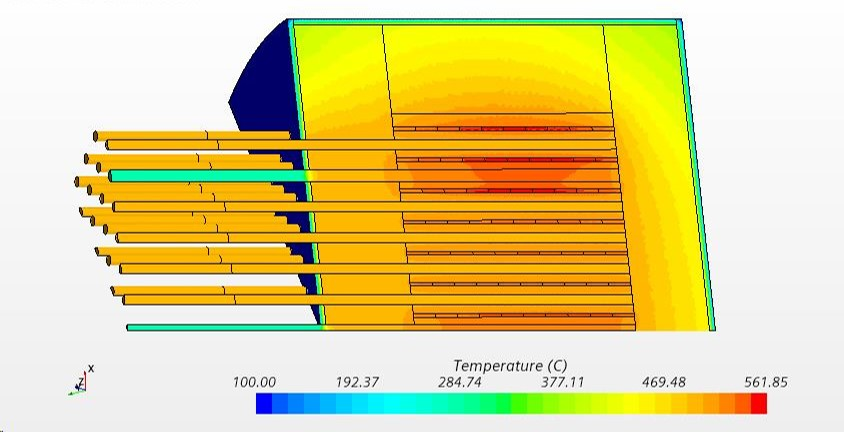
\includegraphics[scale=0.46]{CNBHeatMap.jpg}
  \caption{Multiphysics Heatmap of the Canadian Thermal Battery\textsuperscript{\texttrademark}. }
  \label{fig:mcd}
\end{figure}

When importing figures or any graphical image please verify two things:
\begin{enumerate} 
\item Any number, text or symbol is in Times font and is not smaller than 
  10-point after reduction to the actual window in the paper,
\item That it can be translated into PDF.
\end{enumerate}

Numbers up to ten should be spelled out. Numbers of 11 and higher are numerals.

Equations, such as Eq. (\ref{sample_equation}), should be centered and 
sequentially numbered to the flush right of the formula.

\begin{equation}
  \label{sample_equation}
  \mathrm{Speedup}=\frac{1}{\frac{f}{p}+(1-f)},
\end{equation}
where $f$ and $p$ are some variables that need to be explained here.  Note that the equation has a punctuation mark, and the continuation of a paragraph after an equation should not be indented.  
All paragraphs, as well as section or subsection headings, are separated by a 6~pt spacing.

\subsubsection{Sub-subsection level and lower: only first character uppercase}

See Table \ref{table:example} for a sample table.  The ``tabls'' package is
recommended for improved row and column spacing.  Notice the caption appears 
above the table by setting the \verb!\caption! command immediately 
after the \verb!\begin{table}!. Tables are numbered in Roman 
numerals, with the caption centered above the table, in \textbf{boldface}.  
Triple-space before and after the table.

\begin{table}[!htb]
  \centering
  \caption{\bf Parallel Performance for the Sample Problem.}
  \label{table:example} 
  \begin{tabular}{|c|c|c|c|} \hline 
   Number of & Wall-Clock & Speedup & Efficiency \\
   Processors & Time (min)$^a$& (T$_{s}$/T$_{p}$) & (\%) \\ \hline
    \ 1 &  100.0 & \ ---    & ---  \\ \hline
    \ 2 &   52.6 & \ 1.9    & 95.0 \\ \hline 
  \end{tabular}
\end{table}

\section{CONCLUSIONS}

Present the summary and conclusions here.

\section*{NOMENCLATURE}

If variables are extensively used in the text, a Nomenclature section would be helpful to the readers.

\section*{ACKNOWLEDGEMENTS}

Acknowledge the help of colleagues and sources of funding, as appropriate.

\textbf{As an example:} The format for this template was adapted from the \LaTeX\ template for the M\&C 2021
conference, incorporating limited elements from the M\&C 2019 template.  The M\&C 2023 organizing committee
thanks the M\&C 2021 and M\&C 2019 technical committees for this support.

% You can enter a bibliography into the document using either BibTex with the bibliography
% style file "mc2023.bst" found in the template directory or using the standard LaTeX
% thebibliography environment.
\newif\ifusebibtex
\usebibtexfalse
%\usebibtextrue

\ifusebibtex
\setlength{\baselineskip}{12pt}
\bibliographystyle{mc2023}
\bibliography{mc2023}
\else
\setlength{\baselineskip}{12pt}
\begin{thebibliography}{300}
\bibitem{journal} B. Author(s), ``Title, using capitalization'' \emph{Journal Name in Italic}, 
  \textbf{Volume in Bold}, pp. 34-89 (20xx).
\bibitem{proc_paper} C. D. Author(s), ``Article Title,'' \emph{Proceedings of
  Meeting in Italic}, Location, Dates of Meeting, Vol. n, pp. 134-156 
  (20xx).
\bibitem{book} E. F. Author, \emph{Book Title in Italic}, Publisher, City \&
  Country (20xx). 
\bibitem{website} ``Canadian SMR Roadmap,'' \\
  \url{https://smrroadmap.ca/wp-content/uploads/2018/12/Technology-WG.pdf} (2018).
\end{thebibliography}
\fi

\appendix
\gdef\thesection{APPENDIX~\Alph{section}}
\section{Sample Appendix 1}
\label{app:a}
If necessary, include Appendices numbered in upper case alphabetical order. This is \ref{app:a}. 



\end{document}
